\documentclass[11pt]{article}  
\usepackage[left=3.5cm, right=3.5cm, bottom=3cm]{geometry}           
\usepackage[parfill]{parskip}    		
\usepackage{graphicx}
\usepackage{cleveref}
\usepackage[export]{adjustbox}
\usepackage{mathabx}
\usepackage{graphicx}
\usepackage{subfigure}
\usepackage{url}						
\renewcommand{\baselinestretch}{1}
\usepackage[font=footnotesize,labelfont=bf]{caption}
\usepackage{float}
\usepackage[font=scriptsize]{caption}
\usepackage[T1]{fontenc}
\usepackage[font=small,labelfont=bf,tableposition=top]{caption}
% \DeclareCaptionLabelFormat{andtable}{#1~#2  \&  \tablename~\thetable}
% \usepackage{caption}
% \usepackage{subcaption}

% \captionsetup{compatibility=false}



\title{CS5014 - Machine Learning 
\\ \vspace{5mm} \Large P2 - Classification of object colour 
\\ using optical spectroscopy 
\\~\\ Report}
\author{140014952}

\small %\date{}
 
\begin{document}
	\maketitle

	\section{Overview}

		The objectives of this practical were to come up with classification model for binary and multi-class classification problems. This submission investigates both binary and multi-class tasks. The solution python scripts can be found in \textit{/binaryML/} and \textit{/multiclassML/} directories. 

		As later sections suggest, the amount of features it takes to determine the class for each task is very low. This is hypothesized based on input analysis and later machine learning observations support these hypotheses. 

		Final predicted class files are recorded in the appendices section of this report and in directories \textit{/binaryTask/} and \textit{/multiClassTask/}.

	\section{Binary Classification Task}

	\subsection{Cleaning data and Feature extraction}

		As the very first step input data were split into training and testing data with 70-to-30 ratio. The analysis were first done on the training set. Sklearn's \textit{train\_test\_split} was used to do so. Also, a seed was used to ensure the same samples are used every time python notebook is fully executed.

		From observations and further analysis in python, data cleaning was not necessary. Data contains negative and positive values that according to the practical specification make sense. 

		However, a functionality to remove all records with null values in was implemented to ensure that the samples are fully prepared.

	\subsection{Data analysis and Visualization}

		To visualize training data X it was plotted with provided wavelength data that contains information about each feature wave length. Additionally, Y training set was used to indicate visually how colours are distributed and can be distinguished. This gave insights as to which features are likely to be good indicators for predicting the colour. 

		\begin{figure}[H]
			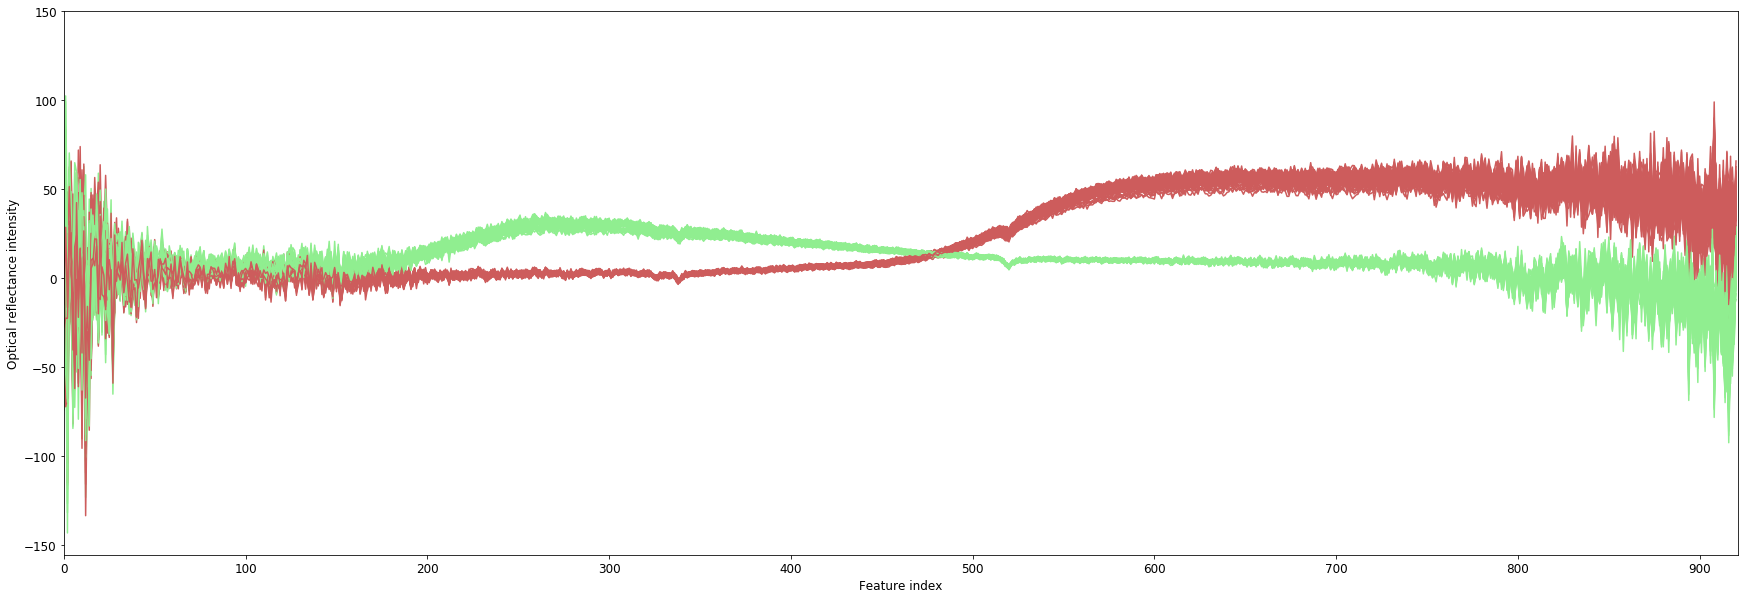
\includegraphics[width=1\textwidth]{png/binary_default}
			\caption{Input feature visualization for binary classification task. Red and green predicting features are indicated by colour.}
			\label{fig:binary}
		\end{figure}

		Fig.\ref{fig:binary} shows that there is a clear distinction between red and green colours in terms of features. From the same figure it can be said that feature values between 420 and 450 wavelengths are more or less shared between both, red and green colours. Around 600 wavelength both colour features overlap. Similarly, towards the final features similar observations can be made. The graph insights suggest that overlapping features are not great for determining the class because a feature value can be shared by both colours therefore reducing possibility of determining the right colour. However, a single feature that is around 530 or 650 should be good enough to determine the class. From fig.\ref{fig:binary} it is clear that intensity at those wavelengths are distinct to each colour.

		The hypothesis therefore is that any feature that distinguishes the two colours at particular wavelength will be good enough to determine the class. According to the fig.\ref{fig:binary} there are many of these features: at wavelengths 500-to-580 and 610-to-720. Therefore, it one feature should be enough to determine the class.

	\subsection{Preparing inputs and Choosing features}

		To choose an appropriate feature an experiment was conducted. A single feature could possibly determine a class therefore a training was done using every single feature separately to determine which one is the most accurate. Fig.\ref{fig:binary_one} shows the results. Y axis represents accuracy score and X axis represents a single feature 0-to-920. 

		\begin{figure}[H]
			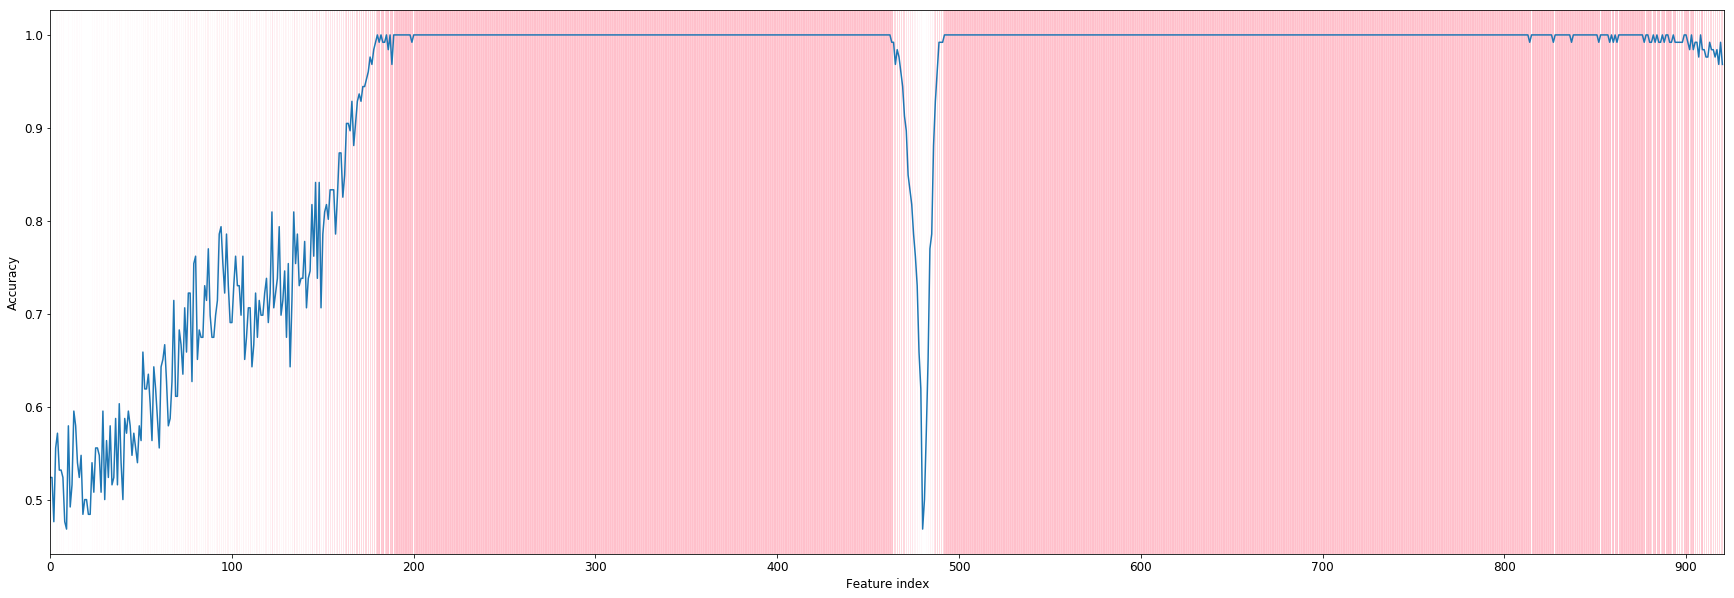
\includegraphics[width=1\textwidth]{png/binary_one}
			\caption{One feature accuracy scores for binary classification.}
			\label{fig:binary_one}
		\end{figure}

		Pink areas cover features that perform very well. It can be seen that features indexed 200-470 and 490 to almost the end of 900 perform with 100\% accuracy. Therefore, any feature that falls in between these boundaries will perform very well. From fig.\ref{fig:}

		From the graphs, large number samples also should not be necessary because there are no noticeable outliers. 

	\subsection{Selecting and Training classification model}
		\subsubsection{Linear logistic regression}
			For binary classification task a simple linear logistic regression model was chosen from sklearn. As expected, the accuracy score is 1.0 with training data. Similar observations are made by using other features too. 

			Once might think that this is caused by over-fitting however from the feature analysis the results make sense. Therefore, scaling which is normally incorporated when over-fitting is suspected was not applied in this situation. 

	\subsection{Evaluating model performance}
		\subsubsection{Linear logistic regression}
			For evaluating performance  

			Tbl.\ref{tbl:binary_test_table} shows results when running the model on test set using four different features. The accuracy score is 100\% in each case as expected. Form the results, it can be said that model works very well on test data when testing on four different occasions, each with different feature: 300, 400, 600 or 700.
			\begin{center}
		  	\begin{table}
		  	\centering
			\begin{tabular}[b]{|c | c|}
				 \hline
				 Feature Index 	 & Accuracy \\ 
 				 \hline
				 300 				& 1.0 	\\ 
				 400 				& 1.0 	\\ 
				 600		 		& 1.0 	\\ 
				 700				& 1.0 	\\ 
				 \hline
			\end{tabular}
			\caption{Accuracy score when testing linear logistic regression model on testing set.}
			\label{tbl:binary_test_table}
			\end{table}
		\end{center}
	\subsection{Result discussion}
		Results seem to be in according to the observations and hypothesis made during data investigation and visualization steps. 

	\section{Multi-Class Task}
		\subsection{Cleaning Data and Feature Extraction}
			Similarly to binary task, no cleaning or feature extraction was necessary.

		\subsection{Data Analysis and Visualization}

			\begin{figure}[H]
				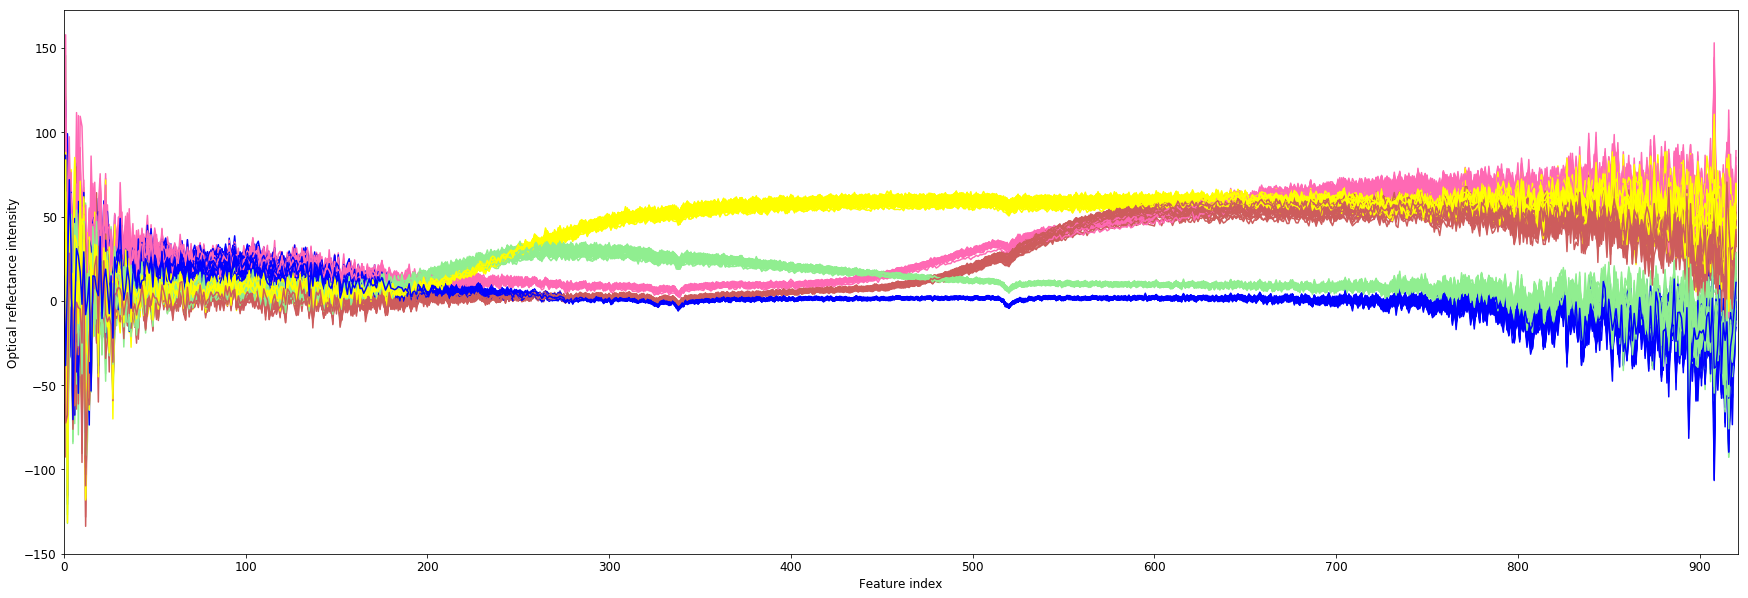
\includegraphics[width=1\textwidth]{png/multi_default}
				\caption{Input feature visualization for multi-class task. Five colour predicting features are indicated by corresponding colour.}
				\label{fig:multi}
			\end{figure}

			Fig.\ref{fig:multi} shows different colour reflectance intensities for five different colours. Green and red just like in binary task are distinct and the same patterns can be recognized in multi-class task. However, due to larger number of colour classes some seem to overlap slightly. From fig.\ref{fig:multi} it can be seen that red and pink colour intensities over different wavelengths are very similar. Yellow on the other hand has very distinct reflectance measures. Just from looking at the graph first two hundred features do not distinct different colours. Blue and green seem to have similar reflectance towards the end. Pink, yellow and red also share similar patterns. 

			From the same graph it can also be seen that some features distinct colours well. For instance, feature indexed 420 is likely to perform well. Since there are almost no overlapping feature values for any of the colours. 

			For instance, when feature 400 is selected histogram in fig.\ref{fig:400_900} shows that the samples are clearly distinctly distributed. WHereas, feature 900 in fig.\ref{fig:400_900} shows that green and blue overlap slightly, red pink and yellow follow the pattern. This also suggest that red and green will be  most likely to be mixed. Pink, red and yellow mixed together too. 

		\begin{figure}
			\hfill
				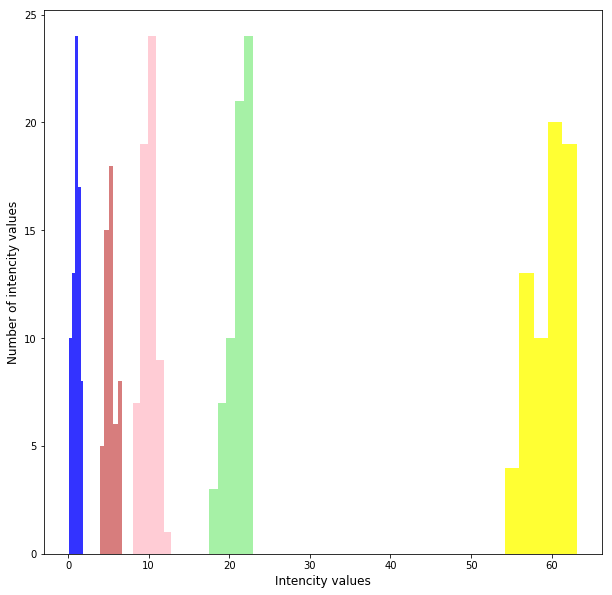
\includegraphics[width=0.4\textwidth]{png/400_multi.png}
			\hfill
				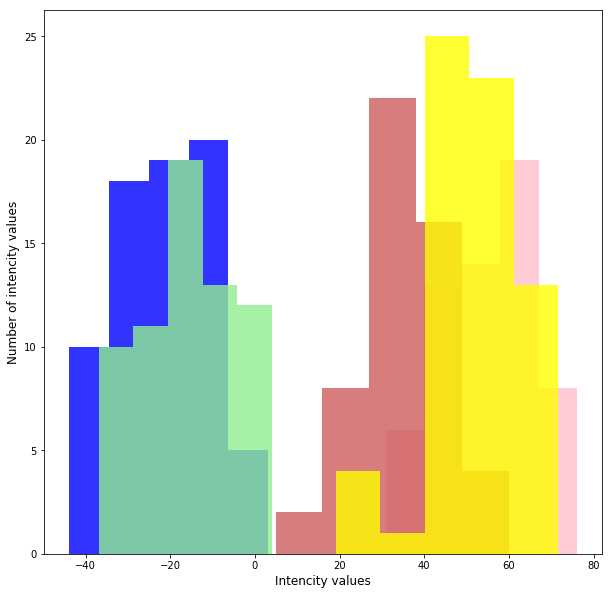
\includegraphics[width=0.4\textwidth]{png/900_multi.png}
			\hfill
			\label{fig:400_900}
			\caption{On the left - feature 400, on the right - feature 900.}
		\end{figure}

		\subsection{Preparing Inputs and Choosing Features}
			\begin{figure}[H]
				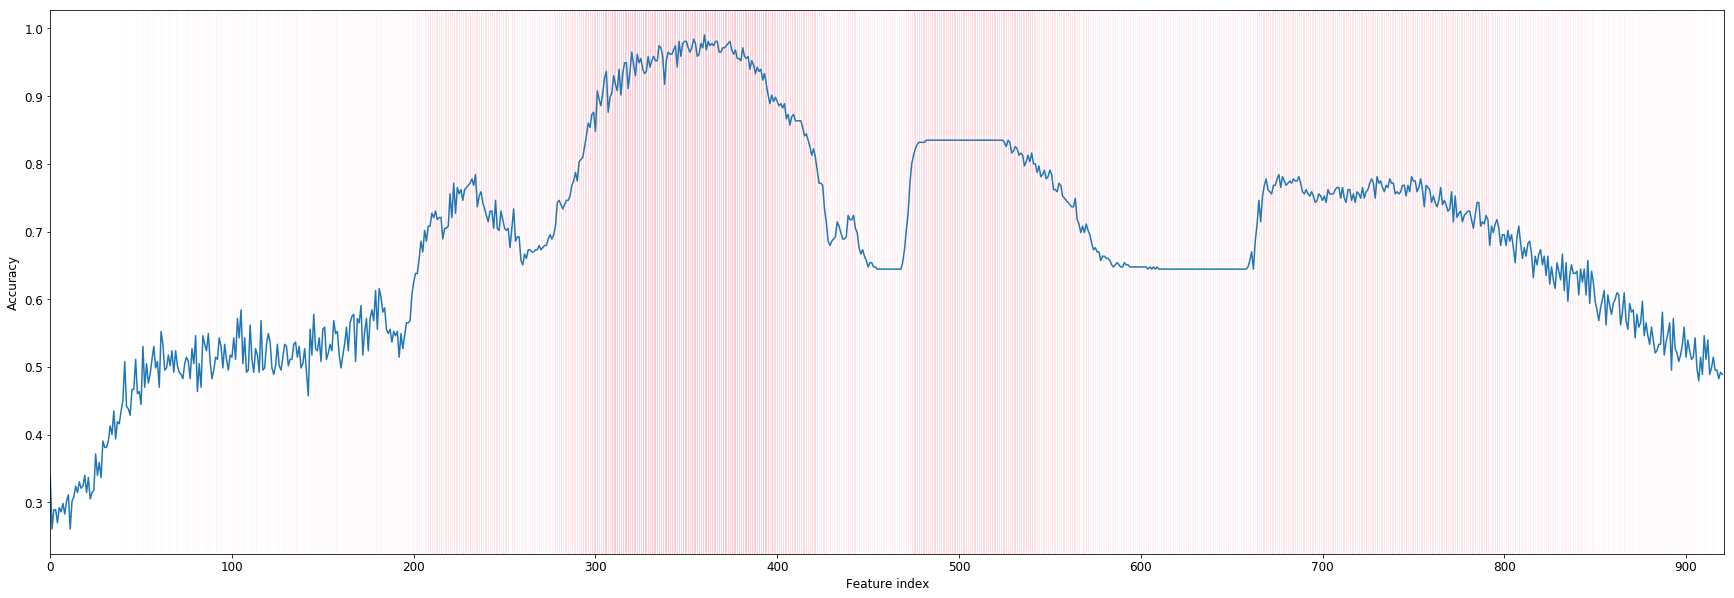
\includegraphics[width=1\textwidth]{png/multi_one}
				\caption{One feature accuracy scores for multi-class classification.}
				\label{fig:multi_one}
			\end{figure}

			Just like in binary task, in order to investigate single feature performance logistic regression model was trained on every feature separately. Fig.\ref{fig:multi_one} demonstrates the results. From the graph it can be seen that some features perform better than other. As per previous input analysis, best accuracy feature are 300-to-400, providing $>$85\% accuracy on training set however not reaching 100\%. Logistic regression model performance is clearly not as great as in binary task. However, still very good. To investigate further and see whether different input combinations provide better accuracy results recursive feature elimination (RFE) algorithm was used form sklearn. The idea behind this selection algorithm is to choose the best features by considering lesser number of them. The result is mask of true and false values that can be used to choose the best feature. 

			For RFE experiment 1-to-10 features were chosen and accuracy scores for each selection were recorded in table .\ref{tbl:accuracy_table}.

		\begin{center}
		  	\begin{table}[h]
		  	\centering
			\begin{tabular}[b]{|c | l | c|}
				 \hline
				 No & Feature Indexes 	  						    & Accuracy \\ 
				 \hline
				 1 & 421 											& 0.810 \\ 
				 2 & 421, 429 										& 0.851 \\ 
				 3 & 421, 429, 250 									& 0.997 \\ 
				 4 & 421, 429, 250, 251 							& 0.997 \\ 
				 5 & 421, 429, 250, 251, 86 						& 1.0 	\\ 
				 6 & 421, 429, 250, 251, 86, 586 					& 1.0 	\\ 
				 7 & 421, 429, 250, 251, 86, 586, 88 				& 1.0 	\\ 
				 8 & 421, 429, 250, 251, 86, 586, 88, 66 			& 1.0 	\\ 
				 9 & 421, 429, 250, 251, 86, 584, 88, 66, 586 		& 1.0 	\\ 
				 10 & 421, 429, 250, 251, 86, 584, 88, 66, 586, 914 & 1.0 	\\ 
				 \hline
			\end{tabular}
			\caption{Accuracy table for different features. }
			\label{tbl:accuracy_table}
			\end{table}
		\end{center}

		This table shows how many features is the optimal number for maintaining good accuracy score. With feature 421 accuracy score is 0.81 which is already very good. As the number of features is increased the accuracy score also becomes even higher. Three features - 421, 429 and 250 are enough to achieve almost 100\% accuracy. Later, as the number of features is more than four the accuracy score is stable and is 1.0.

		Interestingly, the RFE did not choose 350 feature although as the previous experiment suggests it provides over 0.9 accuracy score on its own. 

		\begin{figure}[h]
			\centering
			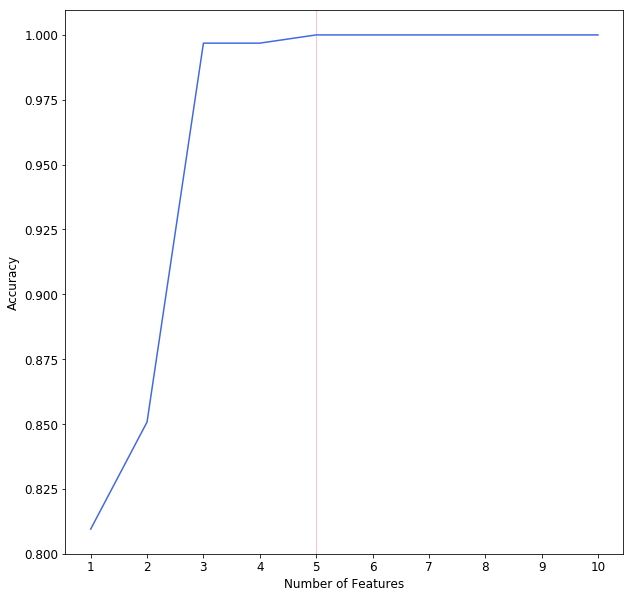
\includegraphics[width=0.5\textwidth]{png/ref_multi}
			\caption{Accuracy depending on number of features extracted by REF.}
			\label{fig:ref_multi}
		\end{figure}
		\subsection{Selecting and Training Classification Models}
		\subsection{Evaluating and Comparing Model Performance}
		\subsection{Result Discussion}
	\section{Conclusion}

	\clearpage
	\appendix
	\section{Appendices}
		\subsection{Binary task results}
		\begin{center}
		  	\begin{table}[h]
		  		\small

		  	\centering
	  	 	% \resizebox{0.2\textwidth}{!}{%

			\begin{tabular}[b]{| c | c|} 
				\hline
				No & Class \\
				\hline
				1 & 1 \\ 2 & 1 \\ 3 & 0 \\ 4 & 0 \\ 5 & 1 \\ 6 & 0 \\ 7 & 0 \\ 8 & 0 \\ 9 & 1 \\ 10 & 0 \\
				\hline
			\end{tabular}
			% }
			\begin{tabular}[b]{| c | c|} 
				\hline
				No & Class \\
				\hline
				11 & 0 \\ 12 & 1 \\ 13 & 1 \\ 14 & 1 \\ 15 & 0 \\ 16 & 1 \\ 17 & 1 \\ 18 & 0 \\ 19 & 1 \\ 20 & 0 \\
				\hline
			\end{tabular}
			\caption{Binary task result for \textit{XToClassify}.}
			\label{tbl:final_binary}
			\end{table}
		\end{center}
		\subsection{Multi-class task results}

\end{document}  